Much of machine learning is concerned with the analysis of given data. By contrast, the fields of optimal experiment design and active learning are concerned with the creation of new data by experimentation or query. In many contexts, careful design of the experiment leads to more efficient learning. The gain in efficiency can be dramatic -- rendering previously infeasible experimental programs feasible. (citation needed)

Idealised active learning can be represented as follows
\begin{center}
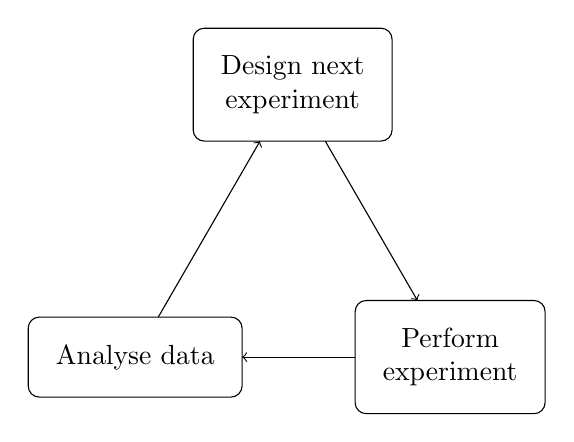
\begin{tikzpicture}
	[every node/.style={inner sep=10,outer sep=0,rounded corners}]
	\node (design) [draw, align=center] at (0, 0) {Design next \\ experiment};
	\node (perform) [draw, align=center] at (2, -3.46) {Perform \\ experiment};
	\node [draw] (analyse) at (-2, -3.46) {Analyse data};
	\draw [->] (design) -- (perform);
	\draw [->] (perform) -- (analyse);
	\draw [->] (analyse) -- (design);
\end{tikzpicture}
\end{center}
It is only within the context of a proposed data analysis that the optimality or suboptimality of an experiment design can be assessed.

\section{Foundations}
\subsection{Problem specification}
We assume the data analysis model for the experiment takes the form given by the graphical model
\begin{center}
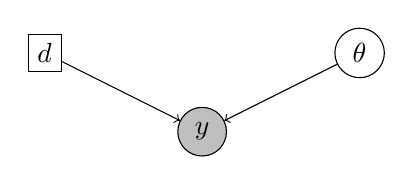
\begin{tikzpicture}
	\tikzstyle{every node}=[draw,shape=circle]
	\node[draw,fill=lightgray] (y) at (0, 0) {$y$};
	\node (t) at (2, 1) {$\theta$};
	\node[draw,shape=rectangle] (d) at (-2, 1) {$d$};
	\draw [->] (d) -- (y);
	\draw [->] (t) -- (y);
\end{tikzpicture}
\end{center}
in which $d$ represents the (non-random) design of the experiment, $\theta$ represents a latent variable and $y$ represents the observed outcome of the experiment. In iterated experiment design, we assume that $\theta$ remains fixed between experiments but $d$ is reselected and $y$ resampled at each experiment. The probabilistic data analysis model is represented by $p(y | \theta, d)$.


\subsection{Criteria for one-step design}
Suppose we assign a real-valued utility $U(y, \theta, d)$ to the event of observing $y$ under design $d$ when the true latent variable was $\theta$. We can average over $y$ to obtain
\begin{equation}
	U(\theta, d) = \int p(y | \theta, d)\ U(y, \theta, d)\ dy
\end{equation}
We can deal with $\theta$ in various ways
\begin{itemize}
	\item The Bayesian approach \cite{chaloner1995} places a prior $p(\theta)$ on $\theta$ and takes $U(d) = \int p(\theta)\ U(\theta, d)\ d\theta$
	\item The minimax approach \cite{fedorov1972} takes $U(d) = \inf_\theta U(\theta, d)$
	\item The local approach \cite{pronzato2010} begins with an estimate $\hat{\theta}$ and sets $U(d) = U(\hat{\theta}, d)$
\end{itemize}
Here, we primarily focus on the Bayesian approach. This is not an arbitrary decision, it can be motivated from decision theoretic considerations \cite{lindley1972}. See \cite{chaloner1995}, \cite{ryan2015} for further discussion of Bayesian experimental design.

Alternatively, we could take the (matrix-valued) `utility'
\begin{equation}
	U(y, \theta, d) = \left( \frac{\partial}{\partial \theta} \log p(y | \theta, d) \right)^2
\end{equation}
which leads to the the Fisher Information Matrix, used in many experiment design criteria \cite{pronzato2010}, defined as
\begin{equation}
	\mathcal{I}(\theta, d) = \int \left( \frac{\partial}{\partial \theta} \log p(y | \theta, d) \right)^2 p(y | \theta, d)\ dy
\end{equation}
We can obtain a scalar utility from $\mathcal{I}(\theta, d)$ by choosing from the `alphabetical' criteria \cite{box1982} which are defined as
\begin{itemize}
	\item D-optimality $U(d, \theta) = \text{det } \mathcal{I}(\theta, d)$
	\item A-optimality $U(d, \theta) = \text{tr } \mathcal{I}(\theta, d)$
	\item E-optimality $U(d, \theta) = \max_i \lambda_i$ where $\lambda_i$ are the eigenvalues of $\mathcal{I}(\theta, d)$
\end{itemize}

Work dating back to \cite{lindley1956} instead uses an information-theoretic utility \footnote{It can also be shown \cite{chaloner1995} that this utility leads to a (modified form) of D-optimality for linear models.}
\begin{equation}
	U(y, \theta, d) = \log \frac{p(\theta | y, d)}{p(\theta)} = \log \frac{p(y | \theta, d)}{p(y|d)}
\end{equation}
and Lindley established that this is the only form that satisfies certain intuitive properties of an informative experiment. For this reason, we will focus on this utility. See \cite{ryan2015} for a fuller discussion of utility functions used in experiment design.

With the information-theoretic utility and Bayesian averaging, we arrive at the following form for $U(d)$, called the \textbf{expected information gain}
\begin{equation}
	U(d) = \eig(d) = \int p(y, \theta | d) \log\frac{p(\theta | y, d)}{p(\theta)} \ dy\ d\theta
\end{equation}
The EIG can be interpreted in a number of ways
\begin{enumerate}
\item As the expectation of information gain. If we define
\begin{equation}
	\text{IG}(y, d) = \text{KL}(\ p(\theta | y, d)\ ||\ p(\theta)\ ) 
\end{equation}
then $\eig(d) = \expect_{y\sim p(y|d)}[\text{IG}(y, d)] $.
\item From APE. Define the \textbf{average posterior entropy} (APE) as 
\begin{align}
	\ape(d) &= \int p(y, \theta | d) \log p(\theta | y, d) \ dy \ d\theta \\
	&= -\int p(y|d) \entropy{p(\theta | y, d)}
\end{align}
where $H$ is the differential entropy.
Then
\begin{equation}
	\eig(d) = \entropy{p(\theta)} - \ape(d)
\end{equation}
and the prior entropy is a constant w.r.t. $d$. Thus EIG maximisation corresponds to APE
minimisation.
\item Mutual information. Recall the mutual information is defined as
\begin{equation}
	\text{MI}(x, y) = \kl{p(x, y)}{p(x)p(y)}
\end{equation}
then we have
\begin{align}
	\text{MI}(y, \theta | d) &= \kl{p(y, \theta | d)}{p(y|d)p(\theta)} \\
	&= \int p(y, \theta | d) \log \frac{p(y, \theta | d)}{p(\theta)p(y|d)} \\
	&= \eig(d)
\end{align}
\item Epistemic uncertainty.
The total entropy or uncertainty in response $y$ is
\begin{equation}
	\entropy{p(y|d)}
\end{equation}
the aleatoric uncertainty under parameter $\theta$ is
\begin{equation}
	\entropy{p(y|\theta, d)}
\end{equation}
Under prior $p(\theta)$, the expected aleatoric uncertainty is
\begin{equation}
	\expect_{\theta \sim p(\theta)}\left[ \entropy{p(y|\theta, d)} \right]
\end{equation}
The epistemic uncertainty, under $p(\theta)$, is
\begin{align}
	&\entropy{p(y|d)} - \expect_{\theta \sim p(\theta)}\left[ \entropy{p(y|\theta, d)} \right] \\
	=&-\int p(y|d)\log p(y|d) + \int p(y, \theta | d)\log p(y|\theta, d)\\
	=& \eig(d)
\end{align}

\end{enumerate}


\subsection{Criteria for multi-step design}
Designing a sequence of multiple experiments, with a view to maximise expected utility can be viewed as a partially observable Markov Decision Process, and falls within the scope of reinforcement learning \cite{pang2018}. The problem is also referred to as backward induction or stochastic dynamic programming. See \ref{sec:oedasrl} for an explicit representation of experiment design as RL. A typical approximate strategy is to optimise the expected utility at each experiment (the greedy strategy), although some have considered non-greedy strategies \cite{gonzalez2016} \cite{pang2018}. See \cite[sec 6.1]{ryan2015} for a summary of backwards induction approaches.

A further complication in multi-step design is optional stopping. 



\subsection{Statistical validity}
References for consistency


\subsection{Applications}
TODO: Major revisions needed

\subsubsection{Machine learning and statistics}
There is long-standing interest in `classical' statistical models and their design \cite{youssefreview}. Consider a basic linear models with Gaussian noise. Optimal design here can be expressed in terms of the eigenspectrum of $XX^T$ (see \cite{chaloner1984}). For nonlinear models, see the section on Physics. What about GLMs? Likely can solve the problem analytically again. These are great baselines. People in the linear models case are often concerned with proving the equivalence of different kinds of optimality \cite{youssefreview}.

In machine learning, experiment design is closely related to two common techniques in, for example, image classification: data augmentation and active learning.

In data augmentation images are rotated, translated, etc to create more training data. We could theoretically optimise the augmentation but this seems wasteful since copying the labels to new images is very easy.

A much more interesting area is \textit{active learning}. In this context, there are a large number of unlabeled images. Labeling is expensive. We select which images to label either up front, or (more typical in active learning) in a sequential manner. The key difference here is that we have a finite pool of unlabeled instances. We may be more interested in reducing uncertainty in the labels of these unlabeled images than in our posterior entropy.

The connection between active learning and Bayesian optimal design was explored in \cite{golovin2010}. In this paper, they start from a place where the outcome of a test is deterministic (think of the 12 men on an island problem). In the noiseless setting, the sequential design can be encoded as a decision tree and the problem is called the Optimal Decision Tree problem. This problem is known to be NP-hard. The OED criterion is introduced later to account for noisy observations and the fact that true parameters need not be known exactly even after all tests have been run.

A particular active learning example can be found in \cite{nowak2009}. We have $\mathcal{H}$ a hypothesis space (read parameter space) and $\mathcal{X}$ a query space (read design space). The goal is to determine the true $h^* \in \mathcal{H}$. Each query outputs a label in $\{-1, 1\}$ corrupted with Bernoulli noise (independent between queries). The algorithm broadly works by targeting $x \in \mathcal{X}$ where the expected posterior label in near $0$ (random guess). The convergence rate of $\prob(\hat{h}_i \ne h^*) \to 0$ is studied (shown exponential). The importance of having access to unlabeled data is exploited by \cite{dasgupta2006}.

\subsubsection{Psychology}
For an overview of optimal experiment design in probabilistic programming, \cite{ouyang2016} from Noah's group is a good place to start. Experiment design is necessary to distinguish competing theories. We should select models with the highest \textit{expected information gain}, written formally as 
\begin{equation}
U(d) = \expect_{(Y, \Theta) \sim p(y, \theta | d)}\left\{\log \frac{p(\Theta | Y, d)}{p(\Theta)}\right\}
\end{equation}
This equation has been studied by mathematical statisticians since the 50's \cite{lindley1956}. We can naively evaluate $U(d)$ in a PPL via \textit{nested inference}.

A canonical experiment discussed in this paper is the 5-4 experiment for category learning \cite{medin1978}. The experiment aimed to distinguish two competing models of category learning: the \textit{exemplar model} (learn categories by comparing new items to all previous items) and the \textit{prototype model} (learn categories by remembering a prototypical example). There are two models, so $\Theta = \{m_1, m_2\}$. During the experiment, participants are presented with a sequence of objects. In the training phase, they are also told the correct label after guessing. In testing they have no feedback. The objects varied in four dimensions: colour, shape, size and count; we can consider the space of objects to be $\{0,1\}^4$. Each object has a label $A$ or $B$. The true labeling mechanism was limited by Medin and Schaffer to be linearly separable. There are 9 inputs in the final testing set and Medin and Schaffer restricted there to be 5 $A$s and 4 $B$s. The objects $0000$ and $1111$ have to be present. Under these restrictions there are 933 possible experiments up to permutation. So $\mathcal{D}$ is a finite set of size 933. $\mathcal{Y}$ is the `test' responses, ie. the subjects responses when they are not given feedback. Thus $\mathcal{Y} = \{A, B\}^9$. The kind of participant numbers seen were 10-30.

In \cite{vincent2017}, the canonical experiment is as follows. We want to model how humans discount future rewards relative to present ones (via utility indifference pricing framework). A single experiment takes the following form: `Would you prefer £$A_1$ at time $t_1$ or £$A_2$ at time $t_2$'? The parameter of interest is the discount factor. Formally, $\mathcal{D} = [0, \infty)^2$, $\mathcal{Y} = \{1, 2\}$ and $\Theta = [0, \infty)$. These three spaces fit together as follows. We first chose $\mathcal{D}$ the space of possible designs. We subsequently chose $\mathcal{Y}$ the space of possible outcomes. We posited a probabilistic model for $Y$ in terms of parameters $\theta$. Focus on non-nested estimation for finite $\mathcal{Y}$ and sequential design. Sequential design means different participants will be asked different questions based on their previous answers.

\subsubsection{Bioinformatics}

In \cite{vanlier2012}, the authors consider experiment design from the perspective that, with little data, many different parameter settings adequately describe the data. Canonical model. Biochemical network modeled as an ODE.
\begin{align*}
&\dot{x} = f(x, u, p) \\
&\dot{y} = g(x, q) + \xi \\
&x(0) = x_0
\end{align*}
$u$ is the input, $x, y$ are time varying (uncontrolled) with $x$ latent and $y$ observed, $p, q, x_0$ are parameters $\theta$ required to simulate the model and do not depend on $t$, $\xi$ represents measurement noise. We treat $\xi$ as iid Gaussian. The paradigm chosen here is expected variance reduction, as opposed to information gain. (Possibly wrong if people still do that.) The variance is in the posterior predictive density.

\subsubsection{Physics}
In \cite{berg2003}, we begin by discussing `classical' experiment design procedures which assume linear dependence between model and outcome $y = G_{m_0}d$. One can solve this linear equation by least squares, $\hat{d} = G^T(GG^T)^{-1}y$. Define $L = G^T(GG^T)^{-1}$, possibly adding regularization as necessary. Basically, you want to maximize the max eigenvalue of $G$, which is essentially a gradient. The larger gradient, the more informative the experiment. In a linear setting, the gradient does not depend on the true parameter value.

Now consider linear noise but a nonlinear function between parameters and outcomes. For example, the authors took
\begin{equation}
R_p = \left(\frac{1}{2}[1 + \tan^{-1} i] - 4c^2 \sin^2 i\right) \frac{\Delta \alpha}{\alpha}
\end{equation}
where $\alpha = (\alpha 1 + \alpha2)/2$, $\Delta \alpha = (\alpha 2 - \alpha 1)$. The parameter we want to optimize is $\alpha2$.

This is a relatively simple and comprehensible case.